% !TEX root = ../intro-stellar-physics.tex
Computing is now ubiquitous in science and technology, and forms a triad with theory and experiment. Stellar modeling has a long and storied history in this area. Of course, libraries of numerical routines are now widely available, and for research it is far better to use a well-written and well-tested routine than trying to build your own. One still needs to have a basic understanding, however, of how a computational technique works! In this appendix, we wish to give a flavor of a few common numerical techniques. 

\section{Numerical precision}\label{s.numerical-precision}
Before diving into the sea of computational techniques, we need to wade a bit in the shallows of floating-point arithmetic. Numbers are stored in base-2 (binary) format: a sequence of 1's and 0's known as \newterm{bits}. The number of bits in this sequence is fixed\sidenote{On most modern systems the default is 64 bits.}, and the processor and compiler define a particular model\sidenote{Notation used here follows \citet{Metcalf2018Modern-Fortran-}.} to represent numbers.

In symbols, an integer $d$ can be written, using $N$ bits, as
\[
d = (-1)^{s}\times\sum_{k=1}^{N-1} d_{k}2^{k-1}.
\]
Here $s$ is the \newterm{sign bit} and $d_{k} = 0,1$. The largest integer in this representation is $2^{N-1}-1$. For example, suppose we are using $N=4$ bits; one bit is reserved to indicate the sign, and with the remaining 3 bits we represent the positive integers from $0$ to $2^{4-1}-1 = 7$ as
\begin{tabular}{rrrrrrrr}
0 & 1 & 2 & 3 & 4 & 5 & 6 & 7\\
\hline
000 & 001 & 010 & 011 & 100 & 101 & 110 & 111
\end{tabular}.

Real numbers can be modeled\marginnote{The IEEE 754 64-bit model uses 11 bits for representing the exponent $\varepsilon$ and the remaining 53 for the fractional part, known as the \newterm{mantissa}. Because $f_{1}=1$ always, it is not stored to make room for the sign bit.}
as follows: for $x \neq 0$, 
\begin{equation}\label{e.modal-reals}
x = (-1)^{s}\times 2^{\varepsilon}\times \sum_{k=1}^{p} f_{k}\times 2^{-k}.
\end{equation}
Here the exponent $\varepsilon_{\min}\le\varepsilon\le\varepsilon_{\max}$ and $f_{k}=0,1$ with $f_{1} = 1$. For example, if $\varepsilon=-6$ and $f_{k} = 11010000\ldots$ (i.e., $f_{k}=1$ for $k=\{1,2,4\}$ and is 0 otherwise), then
$x = 2^{-6}\times (2^{-1}+2^{-2}+2^{-4}) = 0.0126953125$.

\begin{exercisebox}[Binary representation]
What is the floating point number 10.0 in the model representation, eq.~(\ref{e.modal-reals})? Specify $\varepsilon$ and the $f_{k}$.
\label{ex.binary-representation}
\end{exercisebox}

Using the numerical inquiry functions in Fortran 2018, I wrote a small program to report on the arithmetic on my MacBook Pro (Intel Core i5 processor) for 64-bit floating-point arithmetic. The results are as follows.
\begin{Verbatim}[numbers=none]
     exponent = [-1021, 1024]
       digits = 53
 [tiny, huge] = [ 2.2251E-308, 1.7977E+308]
    precision = 15
      epsilon = 2.2204E-16
\end{Verbatim}
Let's understand what these numbers mean.
First, the exponent, $\varepsilon$ in eq.~(\ref{e.modal-reals}), ranges over $-1021\le\varepsilon\le1024$;%
\marginnote{If you are counting, it may seem that $\varepsilon_{\min}$ should be -1023; however, a couple special values of $\varepsilon$ are reserved to indicate exceptions: \texttt{NaN} (not a number), e.g., $\sqrt{-1}$; $\pm$\texttt{Infinity}, e.g., $1/0$; or underflow---the number is too small to be represented in this model with $f_{1}=1$.}
given this, what is the smallest positive number, \texttt{tiny}, that can be represented by the model (eq.~[\ref{e.modal-reals}])? Since in the model $f_{1}=1$, the smallest representable number has $\varepsilon = \varepsilon_{\min}$ and $f_{k\neq 1} = 0$:
\[\mathtt{tiny} = 2^{\varepsilon_{\min}}\times 2^{-1} = 2^{-1022} = \sci{2.2251}{-308}.\]
What is the largest positive number, \texttt{huge}, that can be represented by eq.~(\ref{e.modal-reals})? This number has $\varepsilon=\varepsilon_{\max}$ and $f_{k}=1,\,\forall k=1,\ldots,p$, and $p = 53$ (\texttt{digits}):
\marginnote{In this expression use the formula for the sum of the geometric series,
\[
\sum_{k=1}^{p}r^{-k} = \frac{1-r^{-p}}{r-1}
\]
with $r=2$.}
\[
\mathtt{huge} = 2^{\varepsilon_{\max}}\times \sum_{k=1}^{53} 2^{-k} = 2^{\varepsilon_{\max}}\times(1-2^{-53}) = \sci{1.7977}{308}.
\]
Finally, we can ask: what is the smallest number that, when added to one, gives a number different than one? The number one is represented with $\varepsilon = 1$ and $f_{k} = 10000\ldots$, i.e., $f_{1}=1$ and $f_{k\neq1}=0$. The next number larger than one that can be represented in the model (eq.~[\ref{e.modal-reals}]) has $f_{k} = 10000\ldots00001$; that is, $f_{1}=f_{p}=1$ and all other $f_{k}=0$. Hence, the closest number to 1.0 that we can model with eq.~(\ref{e.modal-reals}) differs from 1.0 by $\mathtt{epsilon} = 2\times2^{-p} = 2^{-52} = \sci{2.2204}{-16}$; our \verb+precision+ in decimal format is therefore about 15 digits.

\begin{exercisebox}[Spacing of model numbers]
Using the representation of exercise~\ref{ex.binary-representation}, what is the nearest number to 10.0 that can be represented in the model of eq.~(\ref{e.modal-reals})?
\end{exercisebox}

\section{Finding the root of a function}
A common task in computation is to find the root of a function: that is, given a function $f(x)$ defined on an interval $a\le x\le b$ with $f(a)$ and $f(b)$ having opposite signs ($f(a)\times f(b) < 0$), find $r\in[a,b]$ such that $f(r) = 0$.

\subsection{Bisection}
A robust method for finding $r$ is \newterm{bisection}. We find the midpoint $m = (a+b)/2$ and compute $f(m)$ (red dot, left, Fig.~\ref{f.bisection-1}). We then determine the interval---$[a,m]$ or $[m,b]$ in which the root lies. For example, in Fig.~\ref{f.bisection-1}, the root lies in $[m,b]$ since $f(m)$ and $f(b)$ have opposite signs. We thus reset the bounds of our interval---in this case, setting $a=m$---and repeat the process (right, Fig.~\ref{f.bisection-1}).
\begin{figure}
\forcerectofloat
\centering
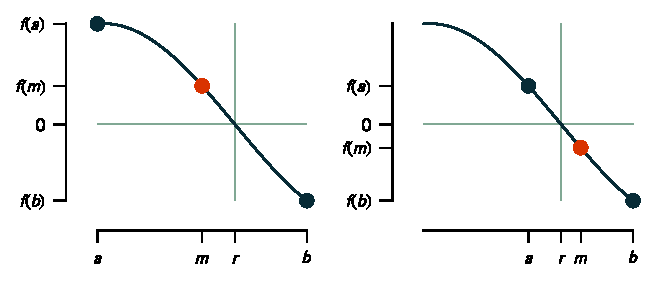
\includegraphics[width=\linewidth]{bisection-1}
\caption[First bisection steps]{During the first iteration (left), we bisect the interval and determine whether the root of the function lies in $[a,m]$ or $[m,b]$.
For the second iteration, we move the left-boundary $a$ to $m$ and compute the next midpoint.
\label{f.bisection-1}}
\end{figure}

\begin{marginfigure}[12\baselineskip]
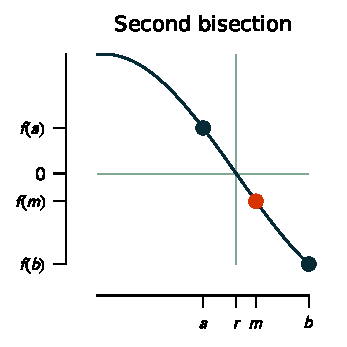
\includegraphics[width=\linewidth]{bisection-2}
\caption[First five bisections]{The first five bisections illustrating the convergence to the root.\label{f.bisection-2}}
\end{marginfigure}
On the second iteration, the root is found to lie in $[a, m]$, so for the third iteration, we set $b=m$. The midpoints gradually converge toward the root, as shown in Fig.~\ref{f.bisection-2}. 
The midpoint represents the current best estimate for the root; the uncertainty in this estimate is given by the width of the interval $\Delta = |b-a|$.
On each iteration this uncertainty in our root is halved: if the uncertainty at the start is $\Delta_{0}$, then after one iteration the uncertainty is $\Delta_{0}/2$; after two iterations, $\Delta_{0}/2^{2}$; after $n$ iterations, $\Delta_{0}/2^{n}$. If our desired \newterm{tolerance} is $\epsilon$---that is, the root is known to lie in an interval of width $\epsilon$---then we should stop iterating when $2^{-n}\Delta_{0} < \epsilon$, or after
\[
	n > \log_{2}\left(\frac{\Delta_{0}}{\epsilon}\right)\;\textrm{iterations.}
\]
Note the $\log_{2}$: on each iteration, we gain another bit of precision on the root. Since our precision is limited to roughly 53 bits (\S~\ref{s.numerical-precision}), this sets the upper limit on how many iterations we need, depending on the initial width of our bracket.

\subsection{Newton's method}
Bisection is robust: it is guaranteed to converge to a root that is bracketed on some interval $a \le x \le b$. It converges to the root at a rather plodding pace, however, and you might wonder: can we speed up convergence a bit? If we can evaluate the derivative of our function, $f^{\,\prime}(x)$, then a classic method for rapidly converging to a root from a good initial guess is \newterm{Newton's method}.  In this method, on each iteration $n$ with a trial root $x_{n}$, evaluate $f(x_{n})$ and $f^{\,\prime}(x_{n})$. To get the next guess, $x_{n+1}$, for the root, construct a line through $(x_{n},f(x_{n})$ and having a slope $f^{\,\prime}(x_{n})$; and solve for where this line crosses the x-axis:
\begin{eqnarray*}
\frac{f(x_{n})-0}{x_{n}-x_{n+1}} &=& f^{\,\prime}(x_{n}),\\
x_{n+1} &=& x_{n} - \frac{f(x_{n})}{f^{\,\prime}(x_{n})}.
\end{eqnarray*}
Fig.~\ref{f.newton} illustrates the first iteration to determine $x_{1}$ from an initial guess $x_{0}$. We then repeat this process to get $x_{2}$, $x_{3}$, and so on, with each one hopefully ever closer to the root.
\begin{marginfigure}[-10\baselineskip]
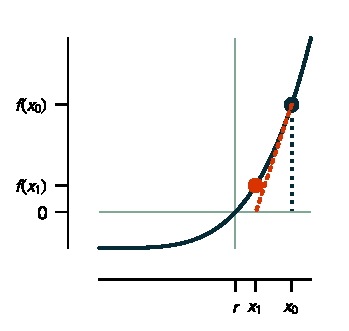
\includegraphics[width=\linewidth]{newton}
\caption[Schematic of Newton's method]{Starting from an initial guess $x_{0}$, we extend a line (red dotted line) of slope $f^{\,\prime}(x_{0})$ to where it crosses $y=0$, thus giving our next guess $x_{1}$.\label{f.newton}}
\end{marginfigure}

Compared with bisection, Newton's method converges quite rapidly: $|x_{n+1}-r| \sim |x_{n}-r|^{2}$---that is, the number of decimal places of precision of the guess roughly \emph{doubles} on each iteration.  Thus, for  $f(x) = x^{4}-4$ with $x_{0}=2$, only 6 iterations\sidenote{that is, $\approx\log_{2}p$ iterations, where $p=53$ is the number of bits of precision, see eq.~(\ref{e.modal-reals})} are needed to find the root to a tolerance $< 10^{-15}$. Nothing comes for free, however; if the initial guess is too far from the root, then Newton's method may converge much slower than bisection, or perhaps not even converge at all (what happens if $x_{0}$ is near the left end of the curve in Fig.~\ref{f.newton}?).
For this reason, Newton's method is generally not preferred.\marginnote{Newton's method is useful for quickly estimating roots of numbers: for example, given a guess $x_{n}$ for a square root of a number $r$, an improved estimate is $x_{n+1} = (x_{n}^{2} + r)/(2x_{n})$. Often one can do one or two iterations mentally and thus estimate the root within a percent or so. For example, to estimate $\sqrt{2}$: $x_{0} = 1$; $x_{1} = 3/2$; and $x_{2} = 17/12$, which is accurate to 0.2\%.}

\subsection{Brent's method}
\newterm{Brent's method}\cite{Brent1973Algorithms-for-} is a rapidly converging, robust routine for finding roots. Like bisection, it requires that the root be bracketed on an interval $x\in[a,b]$. Rather than use the midpoint as a guess for the root, however, Brent's method instead uses, when possible, either linear or quadratic interpolation (see Box~\ref{sb.interpolation}) to construct the next guess for the root.

\begin{sidebar}[Interpolation]
\label{sb.interpolation}
\noindent Through any two points $(x_{0},y_{0})$, $(x_{1},y_{1})$ with $x_{1}\neq x_{0}$, we can fit a unique line, $y=ax+b$, with
\begin{eqnarray*}
	a &=&  \frac{y_{1}-y_{0}}{x_{1}-x_{0}}\\
	b &=&  \frac{y_{0}x_{1} - y_{1}x_{0}}{x_{1}-x_{0}}.
\end{eqnarray*}
Through any three points $(x_{0},y_{0})$, $(x_{1},y_{1})$, $(x_{2},y_{2})$ with $x_{0}$, $x_{1}$, and $x_{2}$ distinct, we can fit a unique quadratic $q = ax^{2}+bx+c$, with $a,b,c$ determined by the equations
\begin{eqnarray*}
a x_{0}^{2} + b x_{0} + c &=& y_{0}\\
a x_{1}^{2} + b x_{1} + c &=& y_{1}\\
a x_{2}^{2} + b x_{2} + c &=& y_{2}.
\end{eqnarray*}
Continuing, through any 4 distinct points we can fit a polynomial of degree 3: $p_{3}(x) = ax^{3} + bx^{2} + cx +d$; and so on. The formula for a polynomial of degree $N$ passing through $N+1$ distinct points is known as the \newterm{Lagrange polynomial}, 
\begin{eqnarray}
p_{N}(x) &=& \sum_{i=0}^{N} y_{i}\ell_{i}(x),\\
\ell_{i}(x) &=& \prod_{k=0,k\neq i}^{N} \frac{x-x_{k}}{x_{i}-x_{k}}.
\end{eqnarray}
For example,
\begin{eqnarray}
\label{e.lagrange-one}
p_{1}(x) &=& y_{0}\frac{x-x_{1}}{x_{0}-x_{1}} + y_{1}\frac{x-x_{0}}{x_{1}-x_{0}};\\
\label{e.lagrange-three}
p_{2}(x) =&& y_{0}\frac{x-x_{1}}{x_{0}-x_{1}}\cdot\frac{x-x_{2}}{x_{0}-x_{2}} 
	+ y_{1}\frac{x-x_{0}}{x_{1}-x_{0}}\cdot\frac{x-x_{2}}{x_{1}-x_{2}}\nonumber\\
	&&+ y_{2}\frac{x-x_{0}}{x_{2}-x_{0}}\cdot\frac{x-x_{1}}{x_{2}-x_{1}};\\
\label{e.lagrange-four}
p_{3}(x) =&&  y_{0}\frac{x-x_{1}}{x_{0}-x_{1}}\cdot\frac{x-x_{2}}{x_{0}-x_{2}}\cdot\frac{x-x_{3}}{x_{0}-x_{3}} \nonumber\\
      &+& y_{1}\frac{x-x_{0}}{x_{1}-x_{0}}\cdot\frac{x-x_{2}}{x_{1}-x_{2}}\cdot\frac{x-x_{3}}{x_{1}-x_{3}} \nonumber \\
      &+& y_{2}\frac{x-x_{0}}{x_{2}-x_{0}}\cdot\frac{x-x_{1}}{x_{2}-x_{1}}\cdot\frac{x-x_{3}}{x_{2}-x_{3}} \nonumber\\
      &+& y_{3}\frac{x-x_{0}}{x_{3}-x_{0}}\cdot\frac{x-x_{1}}{x_{3}-x_{1}}\cdot\frac{x-x_{2}}{x_{3}-x_{2}}.
\end{eqnarray}
\end{sidebar}

\begin{marginfigure}[-12\baselineskip]
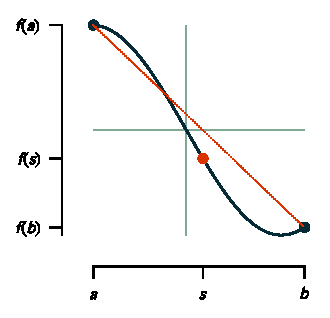
\includegraphics[width=\linewidth]{brent-0}
\caption[Brent's method]{A secant (thin red line) is constructed through the endpoints of an interval containing the root; where this secant crosses the x-axis is used as the next guess (red dot) for the root.\label{f.brent-0}}
\end{marginfigure}
Fig.~\ref{f.brent-0} shows the first iteration of Brent's method. Our test problem is to find the root of $\sin(x)$ on the interval $[1.3,4.5]$. We orient the interval so that $|f(b)|<|f(a)|$, so that $b$ is the ``best guess'' for the root. We then use eq.~(\ref{e.lagrange-one}) to construct a line, known as a \newterm{secant}, connecting $a$ and $b$ and determine the point $s$ where that line crosses the x-axis. In this example, $s$ becomes the new best guess for the root, so we set $b=s$ and store the previous best guess as $c$.

For the next iteration, we have three points: $a$, $b$ (the current best guess), and $c$ (the previous best guess). We can therefore fit a parabola (Fig.~\ref{f.brent-1}) through the three points $(a,f(a))$, $(b,f(b))$, and $(c,f(c))$, using eq.~(\ref{e.lagrange-three}). Instead of fitting a parabola $y = p_{2}(x)$, however, we fit $x = p_{2}(y)$; the reason is that we can simply set $y=0$ in eq.~(\ref{e.lagrange-three})---with $x,y$ exchanged---to find the next guess.
\begin{marginfigure}[-8\baselineskip]
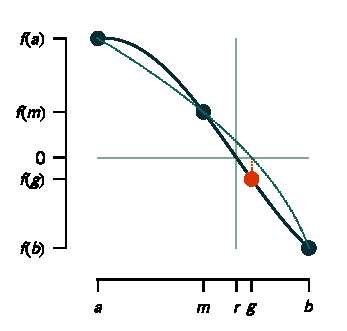
\includegraphics[width=\linewidth]{brent-1}
\caption[Second iteration, Brent's method]{A parabola $x=p_{2}(y)$ (thin red curve) is fit through the previous guesses that bracket a root, and where this parabola intersects $y=0$ is used as the next guess $s$ (red dot) for the root.\label{f.brent-1}}
\end{marginfigure}

The new guess for the root $s$ (Fig.~\ref{f.brent-2}) is on the same side of the root as $a$; hence the previous best guess becomes $a$, and we set $b = s$. We are then ready to perform a linear interpolation to determine the next guess, Fig.~\ref{f.brent-2}. After this third iteration, our new guess $s$ is quite close to the root, $|s-r| = \sci{5}{-4}$. To reach machine precision for this problem took only 6 iterations.
\begin{marginfigure}
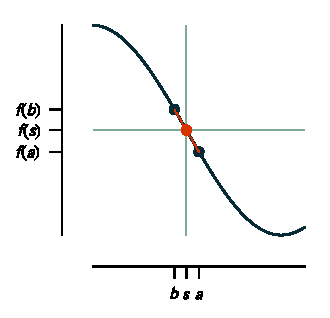
\includegraphics[width=\linewidth]{brent-2}
\caption[Third iteration, Brent's method]{Brent's method is repeated on the restricted interval $[m,b]$ using the points $m,g,b$ to fit a new parabola and determining the next guess (red dot) for the root.\label{f.brent-2}}
\end{marginfigure}

Although the use of linear and quadratic interpolation can converge rapidly, for some cases the interpolation can fail. By keeping track of the previous best guesses for the root, Brent's method can test whether the best guesses for the root are converging as rapidly as bisection. If the guesses aren't improving quickly enough, or if the guess is out of bounds, the method falls back to taking a bisection step. This combination of rapid convergence and robustness makes Brent's method a workhorse routine for finding roots.

\section[Solving a system of ordinary differential equations]{Numerically solving a system of ordinary differential equations}
Another common numerical task is to integrate a system of first-order ordinary differential equations (ODEs). That is, given a system of equations
\begin{equation}\label{e.equation}
\DDt{z} = f(t,z)
\end{equation}
with specified initial conditions $z(t=t_{0})$, find $z(t)$.
Here $z$ is shorthand for an \emph{array} of variables: $z(t) = \{ z_{0}(t), z_{1}(t), z_{2}(t), \ldots\}$. Likewise, $f(t,z)$ is an array of known, specified functions: $f(t,z) = \{f_{0}(t,z), f_{1}(t,z), f_{2}(t,z), \ldots\}$.

A prominent example is Newton's equation of motion,
\begin{equation}\label{e.Newton-2nd}
\frac{\dif^{2}\bvec{r}}{\dif t^{2}} = \frac{\bvec{F}}{m}.
\end{equation}
You may object that this is a second-order differential equation; but notice that if we define
\[
	\bvec{v} = \DDt{\bvec{r}}
\]
then we can recast this single second-order differential equation into a system of two\sidenote{Strictly speaking, this is a system of \emph{six} ODEs: three components of $\bvec{r}$ and three components of $\bvec{v}$.} first-order differential equations of the form (\ref{e.equation}):
\begin{eqnarray}
	\DDt{\bvec{r}} &=& \bvec{v}\\
	\DDt{\bvec{v}} &=& \frac{\bvec{F}}{m}.
\end{eqnarray}

As a worked example, we'll now show how to obtain an approximate numerical solution for the following system of ODEs,
\begin{eqnarray}
\DDt{z_{0}} &=&  2\pi z_{1}\label{e.z0}\\
\DDt{z_{1}} &=& -2\pi z_{0}\label{e.z1},
\end{eqnarray}
with boundary conditions
\begin{equation}\label{e.z-boundary}
	z_{0}(t=0) = 0,\qquad z_{1}(t=0) = 1.
\end{equation}
The solution to equations (\ref{e.z0})--(\ref{e.z1}) is
\begin{eqnarray}
z_{0} &=& \sin(2\pi t),\label{e.z0-sol}\\
z_{1} &=& \cos(2\pi t).\label{e.z1-sol}.
\end{eqnarray}
as you can easily verify.

\newthought{Suppose we know $z(t)$ at some point $t$} and we wish to make a numerical estimate of $z$ at a nearby point $t+h$. We have the values of $z$ and we therefore wish to implement eq.~(\ref{e.equation}) 
for equations~(\ref{e.z0})--(\ref{e.z1}) into a single function.

\begin{sidebar}[Functions]
What is a function in the context of a program? Basically, a function is a self-contained group of statements that you name. For example, to implement $\dif z/\dif t = f(t,z)$ for equations~(\ref{e.z0})--(\ref{e.z1}), we might write (in Python)
\begin{Verbatim}[numbers=none]
def f(t,z):
    """
    RHS of equation dz/dt = f(t,z)
    """
    # this makes an array of length 2,
    # each element of which is zero
    dzdt = np.zeros(2)

    # equation (A.5)
    dzdt[0] = 2.0*np.pi*z[1]
    # equation (A.6)
    dzdt[1] = -2.0*np.pi*z[0]
    return dzdt
\end{Verbatim}
In this listing we give our function the uninspired name \code{f}. A function may receive information, which is listed in the parentheses after the function name: \code{(t,z)}. Thus, the first line
\begin{Verbatim}[numbers=none]
def f(t,z):
\end{Verbatim}
says ``bundle the following list of statements together and call it \code{f}. The statements expect as input two variables, called \newterm{arguments}, which will be referred to in the function as \code{t} and \code{z}.''
This function then does three things: it creates an array \code{dzdt} of length 2, sets the first element of this array to \code{2.0*np.pi*z[1]}, and sets the second element to \code{-2.0*np.pi*z[0]}. The final statement
\begin{Verbatim}[numbers=none]
    return dzdt
\end{Verbatim}
says ``finish, and provide the value of \code{dzdt}'' to whatever \newterm{called} the function. Thus, for example, after defining the function, you could write
\begin{Verbatim}[numbers=none]
k = f(x,y)
\end{Verbatim}
where \code{x} and \code{y} are variables you had already defined.
Python would interpret this as: ``Execute the statements in the function \code{f}. In those statements, set the value of \code{t} to be that of \code{x} and the value of \code{z} to be that of \code{y}. After executing those statements, store the value of the function variable  \code{dzdt} in \code{k} and carry on.''
\end{sidebar}

With the definition of a function $f$, we can compute the right-hand side of equation~(\ref{e.equation}). Our problem can thus be stated as follows:
given $z(t)$, construct an estimate for $z(t+h)$. If we can do this, then we can advance the solution stepwise from the initial condition $z(t=t_{0})$. We'll now present three algorithms for doing so, starting with the least accurate. Our example will use $t=h=0.12$; Fig.~\ref{f.solution} shows the solution for $z_{0}(t)$ over this interval.
\begin{marginfigure}
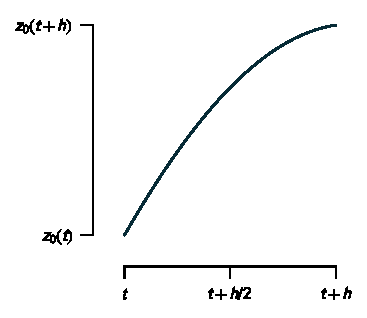
\includegraphics[width=\linewidth]{solution}
\caption[Solution for a sample set of ODE's]{\label{f.solution} Solution (\ref{e.z0-sol}) for $z_{0}$ in the system of equations (\ref{e.z0})--(\ref{e.z1}) from $t=0.12$ to $t+h=0.24$.}
\end{marginfigure}

\subsection{Forward Euler}

The first, and simplest, method goes back to Euler.
Suppose at time $t$ we know the solution $z(t)$ to eq.~(\ref{e.equation}). We can expand $z(t)$ as a Taylor series about this point to obtain
\[ z(t+h) = z(t) + h \left.\frac{\dif z}{\dif t}\right|_{t} + \frac{h^{2}}{2!} \left.\frac{\dif^{2} z}{\dif t^{2}}\right|_{t} + \ldots \]
But $\dif z/\dif t = f(t,z)$ is a known function. So to $\mathcal{O}(h^{2})$,
\begin{eqnarray}
	z(t+h) &\approx& z(t) + h \left.\frac{\dif z}{\dif t}\right|_{t}. \nonumber\\
		&=& z(t) + h \left.f(t,z)\right|_{t}.
\label{e.fEuler}
\end{eqnarray}
Figure \ref{f.forward-Euler} displays a schematic of a forward Euler step. We first compute the slope $f(t,z)$ and then use this to extend the solution to a point $t+h$. By repeating this step over and over, we can march our solution along.
\begin{marginfigure}
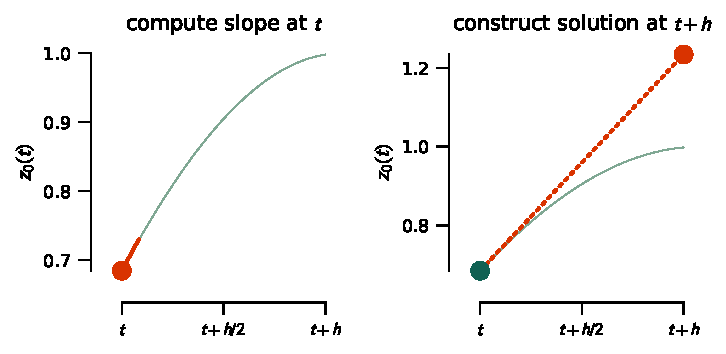
\includegraphics[width=\linewidth]{forward-Euler}
\caption[Schematic of a single forward Euler step]{\label{f.forward-Euler}Schematic of a single forward Euler step, in which we compute the slope $f(t,z)$ and extrapolate the solution from $t$ to $t+h$.}
\end{marginfigure}

How accurate is this \newterm{forward Euler} algorithm? From its definition, the error on each step comes from truncating the Taylor series and is $\mathcal{O}(h^{2})$. What do we mean by this? For sufficiently small $h$, reducing the step by a factor of 2 should reduce the error in a single step by a factor of 4. Another way to put this is that the forward Euler reproduces $z(t)$ exactly if $z$ is a linear function of $t$.
Unfortunately, errors tend to compound with each step, and the smaller the stepsize, the more steps are required. To integrate over a fixed interval $T$ takes $T/h$ steps; if the error on a given step is $\mathcal{E}\sim \mathcal{O}(h^{2})$, then the total integration error will be something like $T/h \times \mathcal{E} \sim \mathcal{O}(h)$.  We therefore call this forward Euler method a \textbf{first-order} method. Reducing the stepsize by a factor of 2 only reduces the integration error by a factor of 2.

\subsection{Second-order Runge-Kutta}

The forward Euler algorithm is not accurate unless the step size $h$ is kept small; as a consequence, a large number of steps are required, which is computationally inefficient. We can improve efficiency if the numerical solution agreed with the solution's Taylor series to a higher order in $h$.
\begin{exercisebox}[Second-order Adams-Bashforth method]
Suppose we have managed to construct a sequence of numerical solutions $\phi_{n}$ to the ODE, eq.~(\ref{e.equation}), such that $\phi_{n} = z(t_{n}=n\times h)$. To find the solution $\phi_{n+1}$ at $t_{n+1}=(n+1)h$, we write $\phi_{n+1}$ in terms of the solutions at $t = t_{n}$ and $t=(n-1)h$:
\begin{equation}\label{e.adams-bashforth}
\phi_{n+1} = \phi_{n} + h\left[af(t_{n},\phi_{n}) + bf(t_{n-1},\phi_{n-1})\right].
\end{equation}
Find the parameters $a$ and $b$ such that $\phi_{n+1}$ agrees with $z(t_{n+1})$ to second order in $h$, that is, so the truncation error is $\mathcal{O}(h^{3})$. Equation~(\ref{e.adams-bashforth}) is called the \newterm{second-order Adams-Bashforth method}.
\end{exercisebox}

\begin{figure}
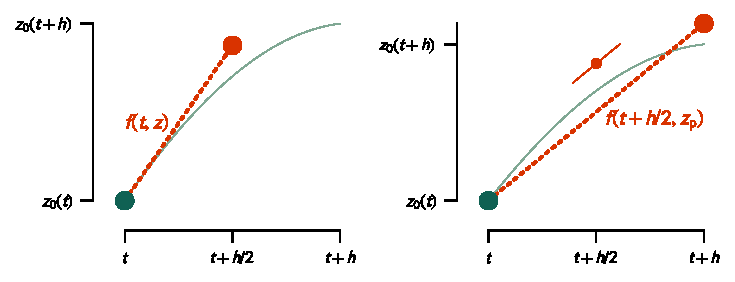
\includegraphics[width=\linewidth]{rk2}
\caption[The second-order Runge-Kutta method]{\label{f.rk2}
In the first stage of a second-order Runge-Kutta step (left), we compute the slope $f(t,z)$ and extrapolate the solution to the midpoint $t+h$; in the second stage (right), we compute the slope of our approximate midpoint solution $f(t+h/2,z_{\mathrm{mp}})$ (left) and use this slope to extend the solution across the interval $[t,t+h]$.}
\end{figure}

A higher-order method stars with using forward Euler to take a step to the midpoint of the interval (Fig.\ref{f.rk2}, left),
\begin{equation}\label{e.predictor}
z_{\mathrm{mp}}\left(t+\frac{h}{2}\right) = z(t) + \frac{h}{2}f[t,z(t)].
\end{equation}
Here $z_{\mathrm{mp}}$ is our estimate of the solution at $t+h/2$.
We then compute the derivative $f$ at $t+h/2$, $z_{\mathrm{mp}}$, and use this corrected value of $f$ to take a step across the entire interval (Fig.~\ref{f.rk2}, right):
\begin{equation}\label{e.corrector}
z(t+h) = z(t) + h f\left(t+\frac{h}{2},z_{\mathrm{mp}}\right).
\end{equation}
One can show that equations~(\ref{e.predictor}) and (\ref{e.corrector}), which are known as the 
\newterm{second-order Runge-Kutta} method, yield a numerical estimate $z(t+h)$ that agrees with the actual solution to $\mathcal{O}(h^{3})$. When integrating over an interval $T$ and taking $T/h$ steps, the solution then has a global error $\sim\mathcal{O}(h^{2})$. Reducing the stepsize by a factor of 2 reduces the integration error by a factor of 4.

\subsection{Fourth-order Runge-Kutta}

An even better method is the classic \newterm{fourth-order Runge-Kutta} algorithm. In this method, the integration of $z$ from $t$ to $t+h$ is done in four steps, as illustrated in Fig.~\ref{f.rk4}.

\begin{figure}
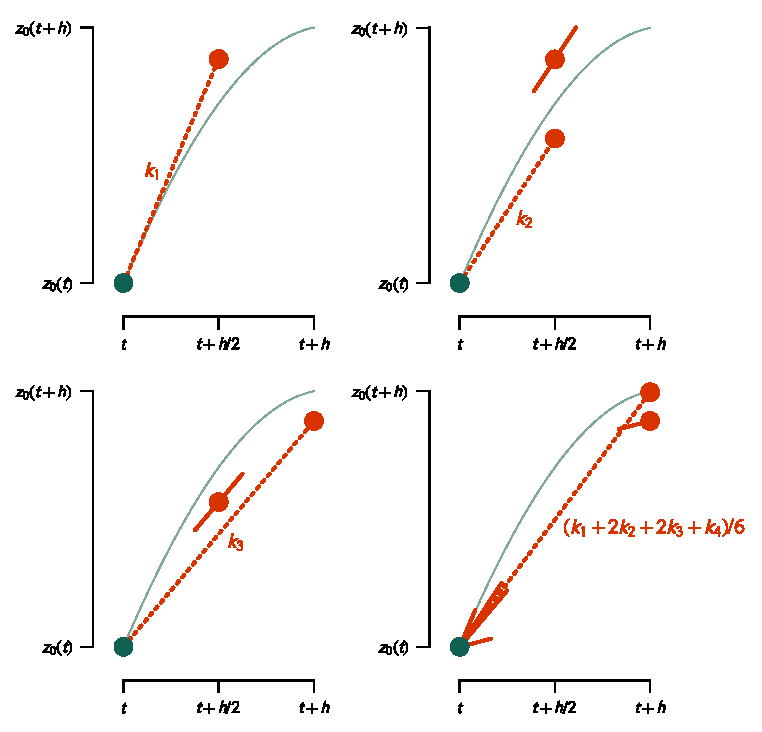
\includegraphics[width=\linewidth]{rk4}
\caption[The fourth-order Runge-Kutta method]{\label{f.rk4}
Stages of the fourth-order Runge-Kutta method.}
\end{figure}

\begin{enumerate}
\item
A forward Euler step with slope $k_{1}$ is taken to the midpoint $t+h/2$ and the solution estimated there (Fig.~\ref{f.rk4}), just as in the second-order method.

\item
This solution at the midpoint is used to make a second estimate of the slope $k_{2} = f(t+h/2,z+k_{1}h/2)$. Using $k_{2}$, we take a new step from $t$ just to the midpoint $t+h/2$ again (Fig.~\ref{f.rk4}).

\item
A new value of the slope $f$ at the midpoint is then computed: $k_{3}=f(t+h/2,z+k_{2}h/2)$. Using $k_{3}$, we then step across the full interval, from $t$ to $t+h$ (Fig.~\ref{f.rk4}).

\item
The slope $k_{4} = f(t+h,z+hk_{3})$ at the endpoint $t+h$ is then computed. The full solution $z(t+h)$ is then constructed from a weighted sum of the $k_{i}$,
\begin{equation}\label{e.rk4}
	z(t+h) \approx z(t) + \frac{h}{6}\left(k_{1} + 2k_{2} + 2k_{3} + k_{4}\right),
\end{equation}
with
\begin{eqnarray*}
k_{1} &=& f(t,z(t)) \\
k_{2} &=& f\left(t+\frac{h}{2}, z(t) + \frac{h}{2}k_{1}\right)\\
k_{3} &=& f\left(t+\frac{h}{2},z(t) + \frac{h}{2}k_{2}\right)\\
k_{4} &=& f\left(t + h, z(t) + hk_{3}\right).
\end{eqnarray*}
\end{enumerate}

Notice that the $k_{i}$ are not independent of one another: each one depends on the intermediate value of $z$ computed in the previous step. The fourth-order Runge-Kutta scheme ``sniffs'' the behavior of $f(t,z)$ over the interval $(t,t+h)$ and constructs a weighted approximation for $\dif z/\dif t$.  One can show that this method produces solutions with a global truncation error $\sim\mathcal{O}(h^{4})$. That is, reducing the stepsize by a factor of 2 should reduce the error by a factor $2^{4} = 16$.

The fourth-order Runge-Kutta scheme is a good general-purpose basic algorithm for integrating systems of ordinary differential equations. It has several limitations, however, three of which we'll discuss here. First, although the truncation error is $\sim\mathcal{O}(h^{4})$, we have no way of knowing \emph{a priori} the size of the error. Integrators with \newterm{adaptive stepsizes} use Runge-Kutta steps with different orders to estimate the size of the error and adjust $h$ to maintain the accuracy to some desired tolerance. Second, the method doesn't know anything about underlying symmetries in the systems of ODEs. \newterm{Symplectic integrators} are constructed so that errors in position and momentum will tend to offset when computing the total energy, so that conservation of energy is maintained to high accuracy. Finally, the methods we in this section are \newterm{explicit}: the solution is advanced using an explicit formula in terms of the current values of $t,z$. For systems with a large dynamical range (e.g., the difference between the dynamical time and Kelvin-Helmholtz time in a star), the steps must be kept quite small, perhaps prohibitively so, to avoid the numerical solution diverging exponentially.

\section{Cubic splines}
The final commonplace numerical task we'll discuss is interpolation of values in a table of data. In stellar physics, this is often done for opacities or equation of state: one computes, or measures, the opacity under a limited set of composition, temperature, and density and tabulates these values. From this table, we then interpolate to obtain values of the opacity at conditions that lie between table entries. Interpolation using polynomials is discussed in Box \ref{sb.interpolation}; in this section we'll illustrate a commonly used interpolation method, cubic splines.

Through any 4 points $(x_{i},y_{i})_{i=0,\ldots,3}$ we can fit a unique cubic polynomial $y=p_{3}(x)$ (eq.~[\ref{e.lagrange-four}]).  Alternatively, we can fit a cubic polynomial between two points $(x_{i},y_{i})$ and $(x_{i+1},y_{i+1})$ if we also specify the first derivatives $k_{i}$ and $k_{i+1}$ at $x_{i},x_{i+1}$: with $m_{i} = (y_{i+1}-y_{i})/(x_{i+1}-x_{i})$ defined as the mean slope across the interval, the cubic polynomial is
\begin{eqnarray}
\lefteqn{q_{i}(x) =   y_{i}\frac{x_{i+1}-x}{x_{i+1}-x_{i}} 
		   + y_{i+1}\frac{x-x_{i}}{x_{i+1}-x_{i}}
		   + \frac{(x-x_{i})(x_{i+1}-x)}{x_{i+1}-x_{i}}} && \nonumber\\
		   && \times\left[\frac{x_{i+1}-x}{x_{i+1}-x_{i}}(k_{i}-m_{i})
		       -\frac{x-x_{i}}{x_{i+1}-x_{i}}(k_{i+1}-m_{i})\right].
\label{e.spline}
\end{eqnarray}
An example of a cubic between $(x_{0},y_{0})$ and $(x_{1},y_{1})$ with $k_{0}=0$ and various $k_{1}$ is shown in Fig.~\ref{f.spline-1}.
\begin{marginfigure}[-16\baselineskip]
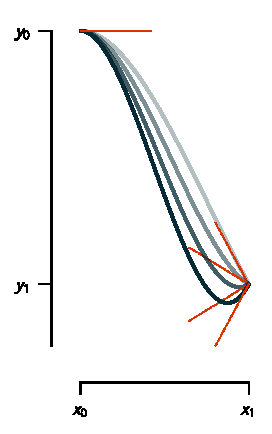
\includegraphics{spline-1}
\caption[Cubic polynomial with varying right-hand slopes]{\label{f.spline-1}Cubic polynomials between points $(x_{0},y_{0})$ and $(x_{1},y_{1})$; the slope at $x_{0}$ is $k_{0}=0$, and the slope $k_{1}$ is varied (red dotted lines).}
\end{marginfigure}

\begin{exercisebox}[Cubic polynomial]
Verify that $q_{i}(x_{i}) = y_{i}$ and $q_{i}(x_{i+1}) = y_{i+1}$ in eq.~(\ref{e.spline}); also verify that $q^{\prime}_{i}(x_{i}) = k_{i}$ and $q^{\prime}_{i}(x_{i+1}) = k_{i+1}$.
\end{exercisebox}

Now suppose we have a sequence of $N+1$ points $x_{0},x_{1},\ldots,x_{N}$ with data values $y_{0},y_{1},\ldots,y_{N}$. On each interval $[x_{i},x_{i+1}]$ we can construct a spline $q_{i}$, subject to the requirement that the splines and their first derivatives are continuous at the interior points. As an example, we take one of the curves from Fig.~\ref{f.spline-1} and cut it into two intervals. We then clamp the derivatives at the endpoints---$k_{0}$ and $k_{2}$---and allow the first derivative at the interior point, $k_{1}$, to vary, with the requirement that the first derivative is continuous at that point (Fig.~\ref{f.spline-2}). The dark curve shows the case where the first derivative is fixed to the value from original spline shown in Fig.~\ref{f.spline-1}.
\begin{marginfigure}[-8\baselineskip]
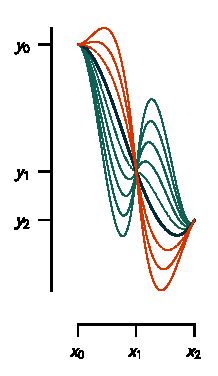
\includegraphics{spline-2}
\caption[Two splines connected at an interior point]{\label{f.spline-2} Two splines spanning $[x_{0},x_{1}]$ and $[x_{1},x_{2}]$, with the slope at the inner point, $k_{2}$, is allowed to vary.}
\end{marginfigure}

As the slope $k_{1}$ is varied, the splines to left and right become more tortuous. The second derivative of the spline characterizes this tight bending. In Fig.~\ref{f.spline-3} we plot the second derivative for three cases: one where $k_{1}$ is fixed to the value from the original spline (solid line), and two with $k_{1}$ less than (dashed line) and greater than (dotted line) this value. Note that in general the second derivative is not continuous at $x_{1}$. In contrast, the original, least contorted, spline does have a continuous second derivative.
\begin{marginfigure}
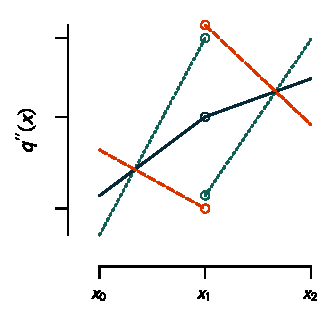
\includegraphics[width=\linewidth]{spline-3}
\caption{\label{f.spline-3} Second derivatives of our spline functions.}
\end{marginfigure}

This motivates constructing a smooth curve by requiring that both the first and second derivatives be continuous at the junction points $x_{1},\ldots,x_{N-1}$. Let's check if this gives us enough conditions. For $N+1$ points $x_{0},x_{1},\ldots,x_{N}$ with data values $y_{0},y_{1},\ldots,y_{N}$, there are $N$ splines: $q_{0}(x)$ on $x_{0}\le x\le x_{1}$, $q_{1}(x)$ on $x_{1}\le x \le x_{n}$, and so on to $q_{N-1}(x)$ on $x_{N-1}\le x\le x_{N}$. Each spline has 4 free parameters, so we have a total of $4N$ parameters. To solve for these parameters, we have the following conditions:
\begin{eqnarray*}
q_{i}(x_{i}) &=& y_{i},\;i=0,\ldots,N-1\qquad\textrm{($N$ conditions)}\\
q_{i}(x_{i+1}) &=& y_{i+1},\;i=0,\ldots,N-1\qquad\textrm{($N$ conditions)}\\
q^{\prime}_{i}(x_{i}) &=& q^{\prime}_{i-1}(x_{i}),\;i=1,\ldots,N-1\qquad\textrm{($N-1$ conditions)}\\
q^{\prime\prime}_{i}(x_{i}) &=& q^{\prime\prime}_{i-1}(x_{i}),\;i=1,\ldots,N-1\qquad\textrm{($N-1$ conditions)}.
\end{eqnarray*}
Our format of the spline, eq.~(\ref{e.spline}), automatically satisfies the first two of these. Adding in the continuity of the first and second derivatives brings us to a total of $4N-2$ equations and leaves us with two free parameters, namely $k_{0}$ and $k_{N}$, the derivatives at the endpoints. We could specify the slopes at the ends (known as a \newterm{clamped spline}), but we usually don't have any way of knowing them \emph{a priori}. A popular choice is to set the second derivative at $x_{0}$ and $x_{N}$ to zero (known as a \newterm{natural} spline).\marginnote{A third choice is the \newterm{not-a-knot} condition, in which we also require the \emph{third} derivative at $x_{1}$ and $x_{N-1}$ to be continuous.}

Let's consider the case of a natural spline. Taking the second derivative of eq.~(\ref{e.spline}) and evaluating at $x=x_{i}$ and $x=x_{i+1}$ gives
\begin{eqnarray}
\label{e.d2spline-left}
q^{\prime\prime}_{i}(x_{i}) &=& -\frac{2}{x_{i+1}-x_{i}}\left[ 2k_{i} + k_{i+1} - 3m_{i} \right];\\
\label{e.d2spline-right}
q^{\prime\prime}_{i}(x_{i+1}) &=& \frac{2}{x_{i+1}-x_{i}}\left[ k_{i} + 2k_{i+1} - 3m_{i} \right].
\end{eqnarray}
Defining $\Delta_{i} = (x_{i+1}-x_{i})^{-1}$ and equating second derivatives at the interior points $x_{i},\,i=1,\ldots,N-1$ then yields the following $N-1$ equations for the $k_{i}$, $i=1,\ldots,N-1$:
\begin{equation}
\Delta_{i-1}k_{i-1} + 2\left(\Delta_{i-1} + \Delta_{i}\right) k_{i} + \Delta_{i}k_{i+1} = 3\left(m_{i-1}\Delta_{i-1} + m_{i}\Delta_{i}\right)
\end{equation}
Setting the second derivatives to zero at $x_{0}$, $x_{N}$ gives the additional equations
\begin{eqnarray}
2k_{0} + k_{1} &=& 3m_{0}\\
k_{N-1} + 2k_{N} &=& 3m_{N-1}.
\end{eqnarray}
This system of equations is termed a \newterm{tridiagonal} system because $i$ contains only $k_{i-1}$, $k_{i}$, and $k_{i+1}$. It can be efficiently solved with two iterations over the equations (see Box~\ref{sb.solving-tridiagonal-system}). After solving for $k_{i}$, if we then wish to interpolate a value $y(x)$, we simply need to find $i$ such that $x_{i}< x < x_{i+1}$ and then insert $x_{i,i+1}$, $y_{i,i+1}$, and $k_{i,i+1}$ into equation (\ref{e.spline}) to interpolate $y(x)$.

\begin{marginfigure}
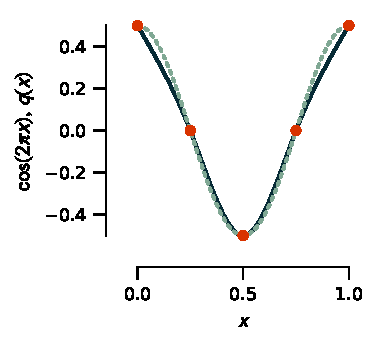
\includegraphics[width=\linewidth]{spline-4}
\caption[Example of a spline fit]{\label{f.spline-4} Spline fit (dotted curve) to the function (solid curve) $\cos(2\pi x)/2$ using 5 evenly spaced points.}
\end{marginfigure}
Fig.~\ref{f.spline-4} illustrates a spline for the function $\cos(2\pi x)/2$ using just 5 points. The largest deviation is at the ends where our imposition of a vanishing second derivative bows the spline (dotted curve) upwards from the true function (solid curve).

\begin{sidebar}[Solving a tridiagonal system]
\label{sb.solving-tridiagonal-system}
These $N+1$ equations for the $N+1$ $k_{i}$ can be written as the matrix equation
\[
\left[\begin{array}{cccccccccc}
	b_{0} & c_{0} \\
	a_{1} & b_{1} & c_{1} \\
%	& a_{2} & b_{2} & c_{2}\\
	& \ddots & \ddots & \ddots \\
	& & a_{i} & b_{i} & c_{i} \\
	& & & \ddots & \ddots & \ddots \\
	& & & & a_{N-1} & b_{N-1} & c_{N-1} \\
	& & & & & a_{N} & b_{N} 
\end{array}\right]
\left[\begin{array}{c}
	k_{0}\\
	k_{1}\\
%	k_{2}\\
	\vdots\\
	k_{i}\\
	\vdots\\
	k_{N-1}\\
	k_{N}
\end{array}\right] = 
\left[\begin{array}{c}
	d_{0}\\
	d_{1}\\
%	d_{2}\\
	\vdots\\
	d_{i}\\
	\vdots\\
	d_{N-1}\\
	d_{N}
\end{array}\right],
\]
with $a_{i} = \Delta_{i-1}$, $b_{i} = 2(\Delta_{i-1}+\Delta_{i})$, $c_{i} = \Delta_{i}$, and $d_{i} = 3(m_{i-1}\Delta_{i-1}+m_{i}\Delta_{i})$, for $i=1,\ldots,N-1$. At the ends, $b_{0}=b_{N}=2$, $c_{0}=a_{N}=1$, $d_{0}=3m_{0}$, and $d_{N}=3m_{N-1}$.
This \newterm{tridiagonal} matrix equation can be efficiently solved as follows.

\begin{enumerate}
\item Divide row 0 by $b_{0}$ so that it becomes%\sidenote{Here we shall denote the row number with a superscript to the left of the row.}
\[
{}^{0}\,\left[\begin{array}{ccccc|c}
  1 & c'_{0} & 0& \ldots & 0 & d'_{0} \end{array}\right]
\]
with $c'_{0} = c_{0}/b_{0}$ and $d'_{0} = d_{0}/b_{0}$.
\item Now we zero out the $a_{i}$ as follows. Assume that we've done this for row $i-1$ and that we already divided row $i-1$ by $b_{i-1}$, so that its diagonal element is 1. Thus rows $i-1$ and $i$ look like
\[
\begin{array}{r} {}^{i-1}\\ {}^{i}\end{array}\,
\left[\begin{array}{ccccccc|c}
	 \ldots & 0 & 1     & c'_{i-1} & 0     & \ldots & \ldots & d'_{i-1}\\
	 \ldots & 0 & a_{i} & b_{i}    & c_{i} & 0      & \ldots & d_{i}
\end{array}\right]
\]
We then multiply row $i-1$ by $a_{i}$ and subtract it from row $i$. This eliminates $a_{i}$:
\[
\begin{array}{r} {}^{i-1}\\ {}^{i}\end{array}\,
\left[\begin{array}{ccccccc|c}
	 \ldots & 0 & 1 & c'_{i-1}            & 0     & \ldots & \ldots & d'_{i-1}\\
	 \ldots & 0 & 0 & b_{i}-a_{i}c'_{i-1} & c_{i} & 0      & \ldots & d_{i}-a_{i}d'_{i-1}
\end{array}\right]
\]
We then divide row $i$ by $b_{i}-a_{i}c'_{i-1}$, giving us
\[
\begin{array}{r} {}^{i-1}\\ {}^{i}\end{array}\,
\left[\begin{array}{ccccccc|c}
	 \ldots & 0 & 1 & c'_{i-1} & 0      & \ldots & \ldots & d'_{i-1}\\
	 \ldots & 0 & 0 & 1        & c'_{i} & 0      & \ldots & d'_{i}
\end{array}\right]
\]
with
\[ c'_{i} = \frac{c_{i}}{b_{i}-a_{i}c'_{i-1}},\qquad d'_{i} = \frac{d_{i}-a_{i}d'_{i-1}}{b_{i}-a_{i}c'_{i-1}}.
\]
We then repeat this with row $i+1$ and march down the rows; this transforms the matrix equation into
\[
\left[\begin{array}{ccccccccccc}
	1 & c'_{0} \\
	 & 1 & c'_{1} \\
	&  & 1 & c'_{2}\\
	& &  & \ddots & \ddots \\
	& & &  & 1 & c'_{i} \\
	& & & &  & \ddots & \ddots \\
	& & & & &  & 1 & c'_{N-1} \\
	& & & & & &  & 1 
\end{array}\right]
\left[\begin{array}{c}
	k_{0}\\
	k_{1}\\
	k_{2}\\
	\vdots\\
	k_{i}\\
	\vdots\\
	k_{N-1}\\
	k_{N}
\end{array}\right] = 
\left[\begin{array}{c}
	d'_{0}\\
	d'_{1}\\
	d'_{2}\\
	\vdots\\
	d'_{i}\\
	\vdots\\
	d'_{N-1}\\
	d'_{N}
\end{array}\right].
\]

\item We now set $k_{N}=d'_{N}$ and then, starting with row $N-1$, we work backwards zeroing out the $c'_{i}$: if row $i$ and $i+1$ are%\marginnote{When we set $c'_{i+1}$ set to zero, we can then equate $k_{i+1}$ with its corresponding entry on the RHS of the matrix equation}
\[
\begin{array}{r} {}^{i}\\ {}^{i+1}\end{array}\,
\left[\begin{array}{ccccccc|c}
	 \ldots & 0 & 1 & c'_{i} & 0 & \ldots & \ldots & d'_{i}\\
	 \ldots & 0 & 0 & 1      & 0 & 0      & \ldots & k_{i+1}
\end{array}\right]
\]
then we multiply row $i+1$ by $c'_{i}$ and subtract it from row $i$ to obtain
\[
\begin{array}{r} {}^{i}\\ {}^{i+1}\end{array}\,
\left[\begin{array}{ccccccc|c}
	 \ldots & 0 & 1 & 0 & 0 & \ldots & \ldots & d'_{i}-c'_{i}k_{i+1}\\
	 \ldots & 0 & 0 & 1 & 0 & 0      & \ldots & k_{i+1}
\end{array}\right];
\]
we then read off $k_{i} = d'_{i}-c'_{i}k'_{i+1}$.
\end{enumerate}
\end{sidebar}
